\phantomsection
\chapter{Results}
\label{chap:eval_results}

\noindent Two kinds of results have been obtained. First results have been obtained by extracting a test set from the KDEF database, and test it against other subjects from the database. Feature extraction is done by LBP, followed by classification using SVM. The second set of results is obtained with the Kinect in real-time conditions, while the entire KDEF database is used for training. The Kinect gets video sequences of a subject in front of it, his or her face being extracted from these sequences using Viola-Jones algorithm. Then the same feature extraction and classification process is applied to these images.
\newline

\phantomsection
\section{First result set}

\vspace{\baselineskip}
\noindent To train the model, 128 face images from the KDEF database have been used for each emotion, plus neutral state. In total, $ 128\times7 = 896 $ face images have been used as train data. To test the system, 12 face images from the KDEF database have been used for each emotion, plus neutral state. In total, $ 12\times7 = 84 $ faces images have been used as test data. For each of these 84 images, face detection was performed first, then the uniform LBP operator extract its features, and then classification is performed using SVM.
\newline

\noindent The model has been trained with different kernels and different parameters. The outcome of these different processes are summed up in Table~\ref{table_results_kernels}. \textbf{\color{red} BLA BLA quel est le meilleur kernel, quelles différences et tout et tout}
\newline

\begin{table}[h]
   \caption{\label{table_results_kernels} Results with different kernels and different parameters}
\begin{tabular}{|c|c|c|c|c|c|c|c|c|}
  \hline
    & Linear & Poly1 & Poly2 & RBF1 & RBF2 & Sigmoid1 & Sigmoid2 \\
  \hline
  neutral & 33.33\% & 33.33\% & 25.00\% & 33.33\% & 33.33\% & 58,33\% & 41.67\% \\
  afraid & 66.67\% & 91.67\% & 100.00\% & 75.00\% & 83.33\% & 75.00\% & 75.00\% \\
  angry & 50.00\% & 50.00\% & 41.67\% & 50.00\% & 50.00\% & 66.67\% & 50.00\% \\
  disgusted & 75.00\% & 83.33\% & 83.33\% & 75.00\% & 75.00\% & 75.00\% & 83.33\% \\
  happy & 91.67\% & 91.67\% & 91.67\% & 91.67\% & 91.67\% & 91.67\% & 91.67\% \\
  sad & 16.67\% & 16.67\% & 8.33\% & 8.33\% & 8.33\% & 8.33\% & 16.67\% \\
  surprised & 33.33\% & 58.33\% & 50.00\% & 66.67\% & 58.33\% & 50.00\% & 75.00\% \\
  overall & 52.38\% & 60.71\% & 57.14\% & 57.14\% & 57.14\% & 60.71\% & 61.90\% \\
  \hline
\end{tabular}
\end{table}

\noindent Poly1 stands for Polynomial and has degree parameter: $ D = 2 $
\newline
\noindent Poly2 stands for Polynomial and has degree parameter: $ D = 3 $
\newline
\noindent RBF1 has cache and $\gamma$ parameters: $ C = 8.0 $ and $ \gamma = 0.0078125 $
\newline
\noindent RBF2 has cache and $\gamma$ parameters: $ C = 32.0 $ and $ \gamma = 0.001953125 $ 
\newline
\noindent Sigmoid1 has cache and $\gamma$ parameters: $ C = 8.0 $ and $ \gamma = 0.0078125 $
\newline
\noindent Sigmoid2 has cache and $\gamma$ parameters: $ C = 32.0 $ and $ \gamma = 0.001953125 $
\newline

\noindent A model has also been trained with same kernels and parameters but using cross-validation (as explained in Chapter \ref{chap:implementation_svm}). Results obtained with a model using cross-validation are compared to those with a model trained normally, this comparison being shown in  Table~\ref{table_results_crossvalidation}. All results are inferior or equal to those without cross-validation, except for linear and sigmoid kernels, with the latter tuned with the second set of parameters. 
\newline

\begin{table}[h]
   \caption{\label{table_results_crossvalidation} Results with and without cross validation}
\begin{tabular}{|c|c|c|c|c|c|c|c|c|}
  \hline
    & with cross validation & without cross validation \\
  \hline
  Linear & 53.57\% & 52.38\% \\
  Poly1 & 54.76\% & 60.71\% \\
  Poly2 & 44.05\% & 57.14\% \\
  RBF1 & 55.95\% & 57.14\% \\
  RBF2 & 50.00\% & 57.14\% \\
  Sigmoid1 & 55.95\% & 60.71\% \\
  Sigmoid2 & 61.90\% & 61.90\% \\
  \hline
\end{tabular}
\end{table}

\noindent \textbf{\color{red} BLA BLA poly kernel et confusion matrix}
\newline 


\begin{table}[h]
   \caption{\label{table_results_confusion_matrix} Confusion matrix}
\begin{tabular}{|c|c|c|c|c|c|c|c|c|}
  \hline
   & neutral & afraid & angry & disgusted & happy & sad & surprised & accuracy \\
  \hline
  neutral & 5 & 4 & 2 & 0 & 1 & 0 & 0 & 41.67\% \\
  afraid & 0 & 9 & 0 & 0 & 0 & 2 & 1 & 75.00\% \\
  angry & 2 & 3 & 6 & 0 & 0 & 1 & 0 & 50.00\% \\
  disgusted & 0 & 1 & 0 & 10 & 0 & 1 & 0 & 83.33\% \\
  happy & 0 & 0 & 0 & 1 & 11 & 0 & 0 & 91.67\% \\
  sad & 0 & 4 & 3 & 1 & 2 & 2 & 0 & 16.67\% \\
  surprised & 2 & 1 & 0 & 0 & 0 & 0 & 9 & 75.00\%\\
  \hline
\end{tabular}
\end{table}

\noindent By looking at the confusion matrix, it is easy to notice that 2 facial expressions are harder to recognize than the others with this system: angry and sad. There is a great difference between these 3 emotions and the 4 other ones (afraid, disgusted, happy, neutral and surprised). Indeed, these 3 emotions are recognized with an accuracy lower than $ 50\% $, while the 4 other ones are recognized with an accuracy equal or higher than $ 75\% $, as summed up in Table~\ref{table_results_accuracy}. Furthermore, the recognition accuracy for the \textit{sad} expression is much lower than random guess, which really contrasts with the \textit{happy} facial expression, the latter reaching a $100\%$ accuracy.
\newline

\begin{table}[h]
   \caption{\label{table_results_accuracy} Recognition accuracy of the six basic emotions and of the neutral state}
\begin{tabular}{|c|c|c|c|c|c|c|c|c|}
  \hline
   $ < 50\% $ & > 75\% \\
  \hline
  neutral ($ 5/12 $) & afraid ($ 9/12 $) \\
  angry ($ 6/12 $) & disgusted ($ 10/12 $) \\
  sad ($ 2/12 $) & happy ($ 11/12 $) \\
   & surprised ($ 9/12 $) \\
  \hline
\end{tabular}
\end{table}

\noindent The numbers in parenthesis represent the number of faces correctly classified over the total number of face images tested.
\newline

\noindent These 6 emotions plus the neutral state can be categorized into 2 groups. Indeed, one group containing the 2 emotions hard to recognize and a second group containing the 2 remaining emotions. The 2 facial expressions \textit{angry}, \textit{sad}, are the ones that distort the less the face. For a same subject expressing these 3 different emotions, as in Figure \ref{kdef_no_difference_emotions}, the differences are not clearly noticeable.
\newline

\begin{figure}[!h]
\begin{center}
\noindent 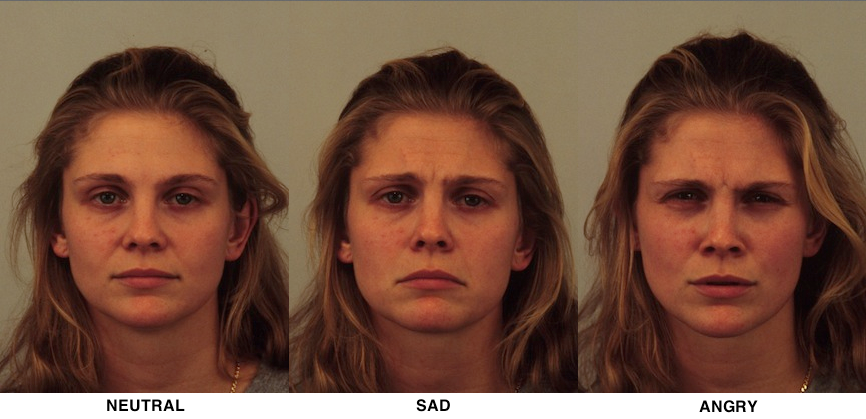
\includegraphics[scale=0.3]{figures/kdef_no_difference_emotions} 
\newline
\caption{Face images from the KDEF database used in the test set}
\label{kdef_no_difference_emotions}
\end{center} 
\end{figure}

\noindent The second group contains the 4 following facial expressions \textit{afraid}, \textit{disgusted}, \textit{happy} and \textit{surprised}. These emotions distort significantly the face when they are expressed. This is why it is easier to recognize them. Figure~\ref{kdef_difference_emotions} shows face images from the KDEF database used in the test set, expressing these 4 facial expressions. Important features carrying emotion as the mouth or the eyes are changing a lot while these 4 emotions are expressed.
\newline

\begin{figure}[!h]
\begin{center}
\noindent 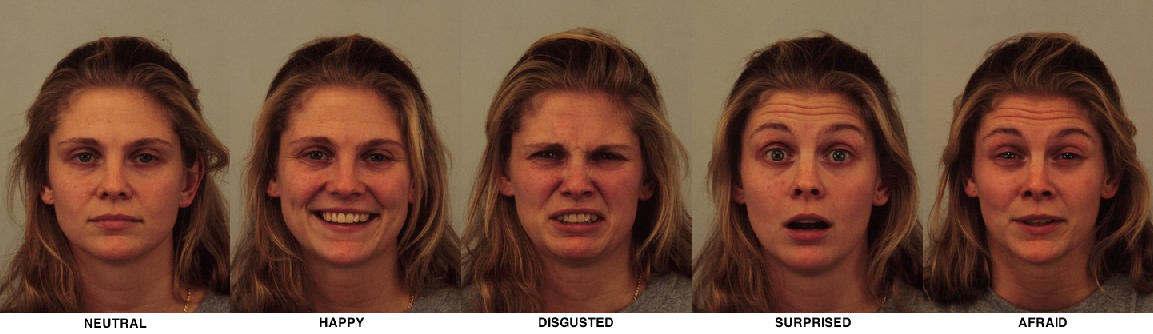
\includegraphics[scale=0.3]{figures/kdef_difference_emotions} 
\newline
\caption{Face images from the KDEF database used in the test set}
\label{kdef_difference_emotions}
\end{center} 
\end{figure}

\noindent As it can be seen in Figure~\ref{kdef_difference_emotions}, for each emotion, eyebrows are raised, eyes are widely opened, and the mouth has a distinct shape, whereas in Figure~\ref{kdef_no_difference_emotions} there are no differences as visible as in Figure~\ref{kdef_difference_emotions}. These variations of intensity might explain twhy the system struggles when trying to differentiate \textit{angry}, \textit{sad} and \textit{neutral} emotional states.
\newline

\phantomsection
\section{Second result set}

\vspace{\baselineskip}
\noindent The second result test is processed in the same way as the first data set, the only difference being the input. Indeed, it is not performed on static images extracted from the KDEF database anymore; images used for texting are extracted from the video stream coming from the Kinect. A subject stands in front of the Kinect, his or her face is detected and extracted, then features are computed, and finally classification is performed. It runs almost in real-time, and the process outputs the name of the emotion expressed.
\newline

\subsection{With face images from the KDEF database}

\vspace{\baselineskip}
\noindent Because the results do not have a good accuracy at first sight, another method is tested. Face images from the KDEF database are printed on A4 paper and are put in front of the Kinect.
\newline

\noindent GIVE THE RESULTS OBTAINED
\newline

\subsection{With subjects}

\vspace{\baselineskip}
\noindent GIVE THE RESULTS OBTAINED
\newline

